
% http://iopscience.iop.org/1367-2630/15/5/053047/

\newcommand{\PaperTitleRecomb}{Recombination effects in soft-x-ray cluster interactions at the xenon giant resonance}

\publication{\PaperTitleRecomb}
\label{section:papers:recomb}

\begin{flushright}
Edward Ackad, Nicolas Bigaouette, Stephanie Mack, \\
Konstatin Popov and Lora~Ramunno
\textit{New Journal of Physics} 15(5), May 2013, 053047\\
\href{http://dx.doi.org/10.1088/1367-2630/15/5/053047}{doi:10.1088/1367-2630/15/5/053047}
\end{flushright}

% Include PDF's abstract in the Table-of-Content as ``subsection 0'' but hide the number
\HidePDFTwoNumbers

\subsection{Author contributions}
The MD package was mostly written by N. B. as was the recombination routines.
The ACI cross-sections were calculated by E. A., who also derived the
recombination rates equations. Original text by E. A. Figures were generated by E. A. with scripts originally written by N. B. but heavily modified.
All authors contributed to the discussion.

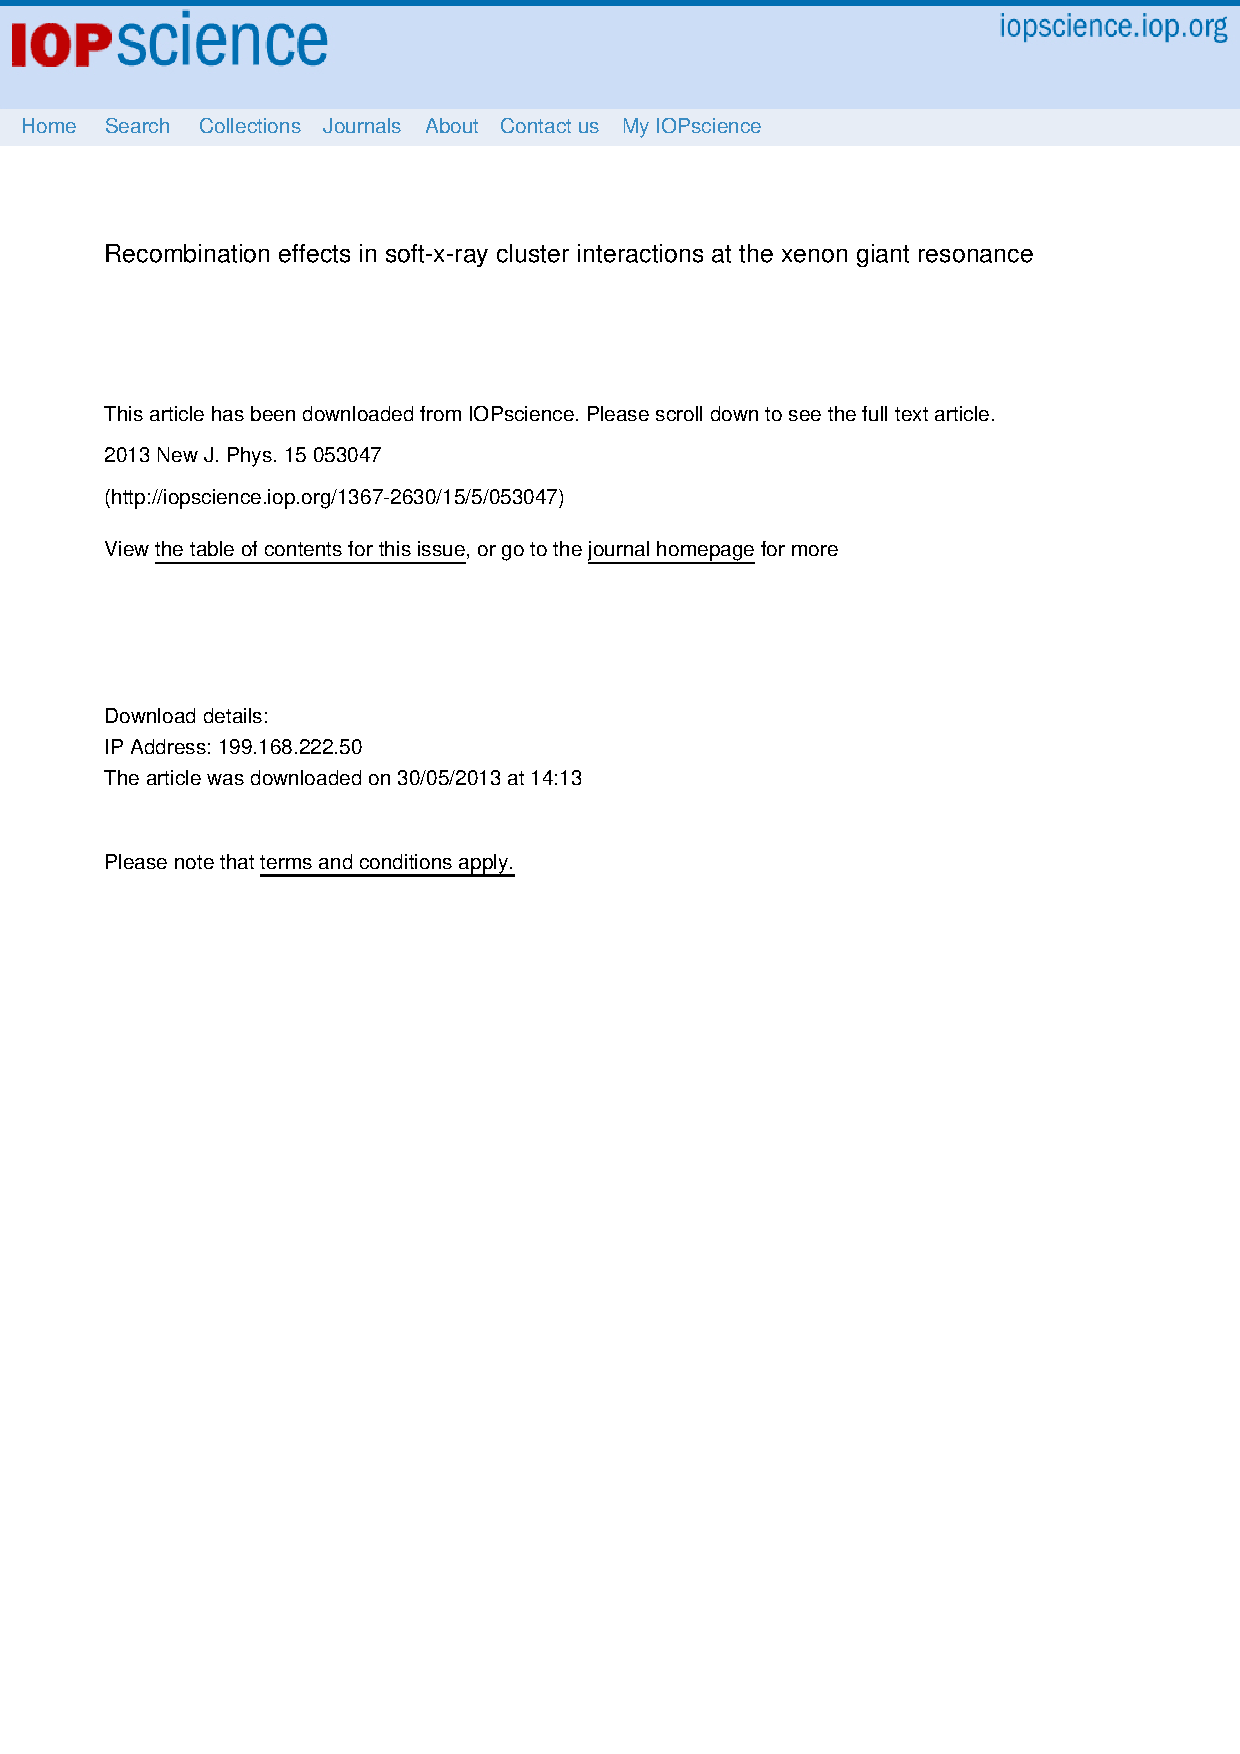
\includepdf[pages=2-,
            addtotoc={
                % Original PDF page, TOC Section hierarchy, # matching TOC level, TOC label, \label{}
                % http://cs.brown.edu/system/software/latex/doc/pdfpages.pdf
                2,subsection,2,Abstract,paper_recomb_abstract,
                3,subsection,2,Contents,paper_recomb_contents,
                3,subsection,2,Introduction,paper_recomb_intro,
                4,subsection,2,Method,paper_recomb_method,
                5,subsubsection,3,Propagation to the detector,paper_recomb_method_propagation,
                6,subsection,2,Recombination in nanoplasmas,paper_recomb_recomb,
                7,subsection,2,Results,paper_recomb_results,
                7,subsubsection,3,Electrons,paper_recomb_results_elec,
                8,subsubsection,3,Ions,paper_recomb_results_ions,
                9,paragraph,4,Time-of-flight signals,paper_recomb_results_ions_tof,
                11,paragraph,4,Total kinetic energy distributions,paper_recomb_results_ions_k_tot,
                13,paragraph,4,Individual kinetic energy distributions,paper_recomb_results_ions_k_ind,
                15,paragraph,4,Relationship between the initial position and final charge state,paper_recomb_results_ions_cs,
                16,subsection,2,Conclusion,paper_recomb_conclusion,
                16,subsection,2,Acknowledgments,paper_recomb_ack,
                16,subsection,2,References,paper_recomb_refs
            }]{papers/Ackad2013_Recomb.pdf}
